\begin{figure}[htbp]
  \centering
  \caption{Distribuição das 30 sementes nas instâncias em que o \texttt{GVNS} estabeleceu novas Melhores Soluções Conhecidas: (a) em \texttt{B/0012} (MSC: $\lvert\mathcal{A}'\rvert = 11$, $\lvert\mathcal{O}'\rvert = 6\,244$), o \texttt{GVNS} supera a MSC em 13 das 30 sementes ($43{,}3\%$), distribuídas em 6 patamares superiores até $6\,252/11 = 568{,}36$; (b) em \texttt{B/0013} (MSC: $\lvert\mathcal{A}'\rvert = 9$, $\lvert\mathcal{O}'\rvert = 6\,813$), o \texttt{GVNS} converge de forma determinística (30/30 sementes) para $6\,814/9 = 757{,}11$, superando a MSC ($757{,}00$) e \texttt{Santos e Baldotto (2025)} ($6\,811/9 = 756{,}78$).}
  \label{fig:novas_msc_sementes}
  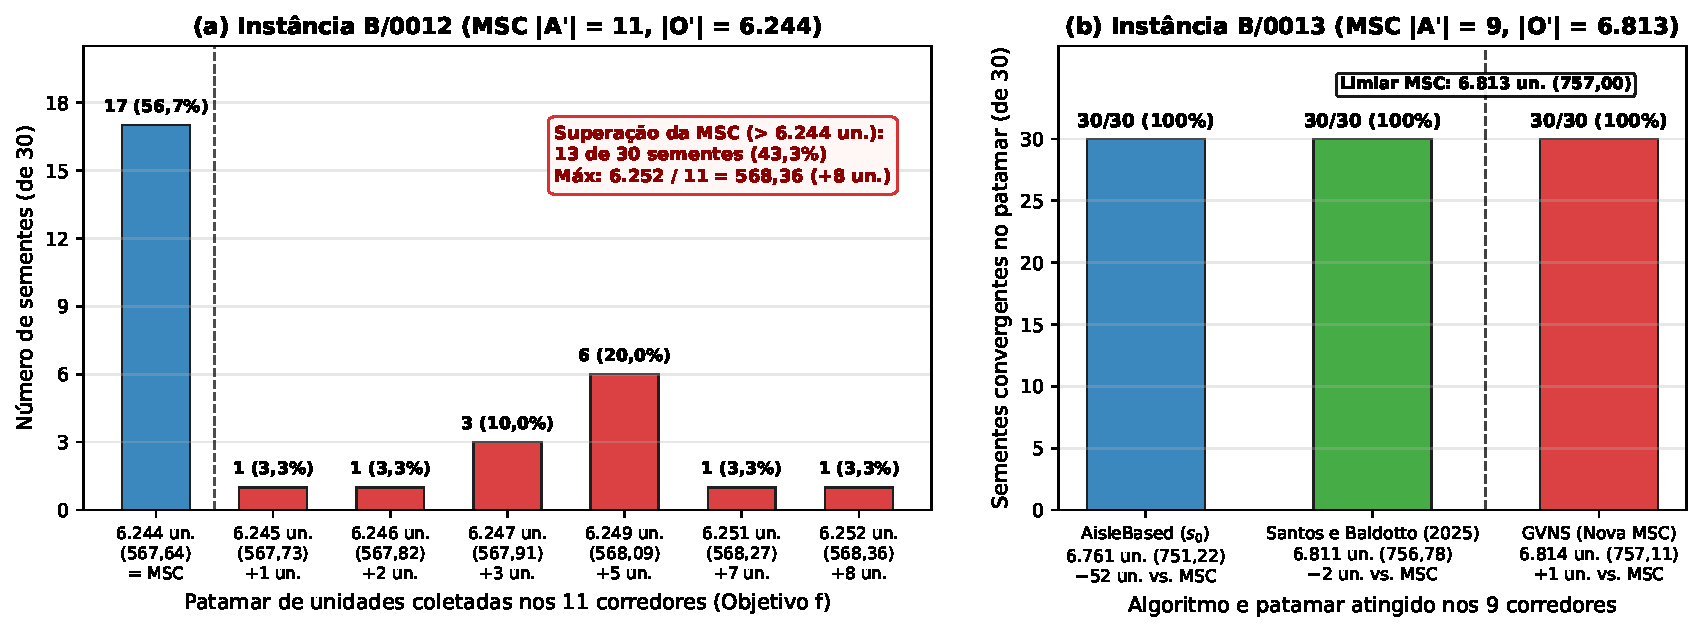
\includegraphics[width=0.95\textwidth]{img/novas_msc_sementes.pdf}
  \caption*{\footnotesize Fonte: Elaborado pelo autor, 2026.}
\end{figure}
